\documentclass[a4paper,11pt]{article}
\usepackage[a4paper, margin=8em]{geometry}

% usa i pacchetti per la scrittura in italiano
\usepackage[french,italian]{babel}
\usepackage[T1]{fontenc}
\usepackage[utf8]{inputenc}
\frenchspacing 

% usa i pacchetti per la formattazione matematica
\usepackage{amsmath, amssymb, amsthm, amsfonts}

% usa altri pacchetti
\usepackage{gensymb}
\usepackage{hyperref}
\usepackage{standalone}

\usepackage{colortbl}

\usepackage{xstring}
\usepackage{karnaugh-map}

% imposta il titolo
\title{Appunti Programmazione Avanzata}
\author{Luca Seggiani}
\date{2025}

% imposta lo stile
% usa helvetica
\usepackage[scaled]{helvet}
% usa palatino
\usepackage{palatino}
% usa un font monospazio guardabile
\usepackage{lmodern}

\renewcommand{\rmdefault}{ppl}
\renewcommand{\sfdefault}{phv}
\renewcommand{\ttdefault}{lmtt}

% circuiti
\usepackage{circuitikz}
\usetikzlibrary{babel}

% testo cerchiato
\newcommand*\circled[1]{\tikz[baseline=(char.base)]{
            \node[shape=circle,draw,inner sep=2pt] (char) {#1};}}

% disponi il titolo
\makeatletter
\renewcommand{\maketitle} {
	\begin{center} 
		\begin{minipage}[t]{.8\textwidth}
			\textsf{\huge\bfseries \@title} 
		\end{minipage}%
		\begin{minipage}[t]{.2\textwidth}
			\raggedleft \vspace{-1.65em}
			\textsf{\small \@author} \vfill
			\textsf{\small \@date}
		\end{minipage}
		\par
	\end{center}

	\thispagestyle{empty}
	\pagestyle{fancy}
}
\makeatother

% disponi teoremi
\usepackage{tcolorbox}
\newtcolorbox[auto counter, number within=section]{theorem}[2][]{%
	colback=blue!10, 
	colframe=blue!40!black, 
	sharp corners=northwest,
	fonttitle=\sffamily\bfseries, 
	title=Teorema~\thetcbcounter: #2, 
	#1
}

% disponi definizioni
\newtcolorbox[auto counter, number within=section]{definition}[2][]{%
	colback=red!10,
	colframe=red!40!black,
	sharp corners=northwest,
	fonttitle=\sffamily\bfseries,
	title=Definizione~\thetcbcounter: #2,
	#1
}

% disponi codice
\usepackage{listings}
\usepackage[table]{xcolor}

\definecolor{codegreen}{rgb}{0,0.6,0}
\definecolor{codegray}{rgb}{0.5,0.5,0.5}
\definecolor{codepurple}{rgb}{0.58,0,0.82}
\definecolor{backcolour}{rgb}{0.95,0.95,0.92}

\lstdefinestyle{codestyle}{
		backgroundcolor=\color{black!5}, 
		commentstyle=\color{codegreen},
		keywordstyle=\bfseries\color{magenta},
		numberstyle=\sffamily\tiny\color{black!60},
		stringstyle=\color{green!50!black},
		basicstyle=\ttfamily\footnotesize,
		breakatwhitespace=false,         
		breaklines=true,                 
		captionpos=b,                    
		keepspaces=true,                 
		numbers=left,                    
		numbersep=5pt,                  
		showspaces=false,                
		showstringspaces=false,
		showtabs=false,                  
		tabsize=2
}

\lstdefinestyle{shellstyle}{
		backgroundcolor=\color{black!5}, 
		basicstyle=\ttfamily\footnotesize\color{black}, 
		commentstyle=\color{black}, 
		keywordstyle=\color{black},
		numberstyle=\color{black!5},
		stringstyle=\color{black}, 
		showspaces=false,
		showstringspaces=false, 
		showtabs=false, 
		tabsize=2, 
		numbers=none, 
		breaklines=true
}


\lstdefinelanguage{assembler}{ 
  keywords={AAA, AAD, AAM, AAS, ADC, ADCB, ADCW, ADCL, ADD, ADDB, ADDW, ADDL, AND, ANDB, ANDW, ANDL,
        ARPL, BOUND, BSF, BSFL, BSFW, BSR, BSRL, BSRW, BSWAP, BT, BTC, BTCB, BTCW, BTCL, BTR, 
        BTRB, BTRW, BTRL, BTS, BTSB, BTSW, BTSL, CALL, CBW, CDQ, CLC, CLD, CLI, CLTS, CMC, CMP,
        CMPB, CMPW, CMPL, CMPS, CMPSB, CMPSD, CMPSW, CMPXCHG, CMPXCHGB, CMPXCHGW, CMPXCHGL,
        CMPXCHG8B, CPUID, CWDE, DAA, DAS, DEC, DECB, DECW, DECL, DIV, DIVB, DIVW, DIVL, ENTER,
        HLT, IDIV, IDIVB, IDIVW, IDIVL, IMUL, IMULB, IMULW, IMULL, IN, INB, INW, INL, INC, INCB,
        INCW, INCL, INS, INSB, INSD, INSW, INT, INT3, INTO, INVD, INVLPG, IRET, IRETD, JA, JAE,
        JB, JBE, JC, JCXZ, JE, JECXZ, JG, JGE, JL, JLE, JMP, JNA, JNAE, JNB, JNBE, JNC, JNE, JNG,
        JNGE, JNL, JNLE, JNO, JNP, JNS, JNZ, JO, JP, JPE, JPO, JS, JZ, LAHF, LAR, LCALL, LDS,
        LEA, LEAVE, LES, LFS, LGDT, LGS, LIDT, LMSW, LOCK, LODSB, LODSD, LODSW, LOOP, LOOPE,
        LOOPNE, LSL, LSS, LTR, MOV, MOVB, MOVW, MOVL, MOVSB, MOVSD, MOVSW, MOVSX, MOVSXB,
        MOVSXW, MOVSXL, MOVZX, MOVZXB, MOVZXW, MOVZXL, MUL, MULB, MULW, MULL, NEG, NEGB, NEGW,
        NEGL, NOP, NOT, NOTB, NOTW, NOTL, OR, ORB, ORW, ORL, OUT, OUTB, OUTW, OUTL, OUTSB, OUTSD,
        OUTSW, POP, POPL, POPW, POPB, POPA, POPAD, POPF, POPFD, PUSH, PUSHL, PUSHW, PUSHB, PUSHA, 
				PUSHAD, PUSHF, PUSHFD, RCL, RCLB, RCLW, MOVSL, MOVSB, MOVSW, STOSL, STOSB, STOSW, LODSB, LODSW,
				LODSL, INSB, INSW, INSL, OUTSB, OUTSL, OUTSW
        RCLL, RCR, RCRB, RCRW, RCRL, RDMSR, RDPMC, RDTSC, REP, REPE, REPNE, RET, ROL, ROLB, ROLW,
        ROLL, ROR, RORB, RORW, RORL, SAHF, SAL, SALB, SALW, SALL, SAR, SARB, SARW, SARL, SBB,
        SBBB, SBBW, SBBL, SCASB, SCASD, SCASW, SETA, SETAE, SETB, SETBE, SETC, SETE, SETG, SETGE,
        SETL, SETLE, SETNA, SETNAE, SETNB, SETNBE, SETNC, SETNE, SETNG, SETNGE, SETNL, SETNLE,
        SETNO, SETNP, SETNS, SETNZ, SETO, SETP, SETPE, SETPO, SETS, SETZ, SGDT, SHL, SHLB, SHLW,
        SHLL, SHLD, SHR, SHRB, SHRW, SHRL, SHRD, SIDT, SLDT, SMSW, STC, STD, STI, STOSB, STOSD,
        STOSW, STR, SUB, SUBB, SUBW, SUBL, TEST, TESTB, TESTW, TESTL, VERR, VERW, WAIT, WBINVD,
        XADD, XADDB, XADDW, XADDL, XCHG, XCHGB, XCHGW, XCHGL, XLAT, XLATB, XOR, XORB, XORW, XORL},
  keywordstyle=\color{blue}\bfseries,
  ndkeywordstyle=\color{darkgray}\bfseries,
  identifierstyle=\color{black},
  sensitive=false,
  comment=[l]{\#},
  morecomment=[s]{/*}{*/},
  commentstyle=\color{purple}\ttfamily,
  stringstyle=\color{red}\ttfamily,
  morestring=[b]',
  morestring=[b]"
}

\lstset{language=java, style=codestyle}

% disponi sezioni
\usepackage{titlesec}

\titleformat{\section}
	{\sffamily\Large\bfseries} 
	{\thesection}{1em}{} 
\titleformat{\subsection}
	{\sffamily\large\bfseries}   
	{\thesubsection}{1em}{} 
\titleformat{\subsubsection}
	{\sffamily\normalsize\bfseries} 
	{\thesubsubsection}{1em}{}

% tikz
\usepackage{tikz}

% float
\usepackage{float}

% grafici
\usepackage{pgfplots}
\pgfplotsset{width=10cm,compat=1.9}

% disponi alberi
\usepackage{forest}

\forestset{
	rectstyle/.style={
		for tree={rectangle,draw,font=\large\sffamily}
	},
	roundstyle/.style={
		for tree={circle,draw,font=\large}
	}
}

% disponi algoritmi
\usepackage{algorithm}
\usepackage{algorithmic}
\makeatletter
\renewcommand{\ALG@name}{Algoritmo}
\makeatother

% disponi numeri di pagina
\usepackage{fancyhdr}
\fancyhf{} 
\fancyfoot[L]{\sffamily{\thepage}}

\makeatletter
\fancyhead[L]{\raisebox{1ex}[0pt][0pt]{\sffamily{\@title \ \@date}}} 
\fancyhead[R]{\raisebox{1ex}[0pt][0pt]{\sffamily{\@author}}}
\makeatother

\begin{document}
% sezione (data)
\section{Lezione del 16-10-25}

% stili pagina
\thispagestyle{empty}
\pagestyle{fancy}

% testo
Ritorniamo sull'argomento dei thread.

Aggiungiamo, rispetto alla scorsa lezione, che ogni thread ha il suo stack (con il suo record di attivazione).
Inoltre, tutti i thread condividono lo stesso heap. Il GC non rimuove gli elementi che sono raggiungibili da qualunque thread.

\subsubsection{Interfaccia Runnable}
Visto che in Java l'ereditarietà è unitaria, dover sempre estendere la classe \textit{Thread} può essere limitante.
In questo Java fornisce l'interfaccia \textit{Runnable}, che quando implementata rende una classe \textit{eseguibile} (come una lambda o un funtore).

Come per la classe Thread, l'interfaccia Runnable è provvista di un metodo astratto \lstinline|run()| da ridefinire per specificarne il comportamento.

Quando si crea un'oggetto \textit{Thread} si può quindi usare un'oggetto che implementa l'interfaccia Runnable come argomento al costruttore:
\begin{lstlisting}[language=java, style=codestyle]	
class MyThread implements Runnable {
	@Override
	void run() {
		System.out.println("Sono un thread");
	}
}

// da qualche altra parte
Thread myThread = new Thread(new MyThread());
myThread.start();

// stampera' "Sono un thread" da un nuovo thread
\end{lstlisting}

\subsection{Stati di un thread}
Un thread può trovarsi in diversi stati, schematizzabili attraverso lo schema (preso direttamente dagli appunti di sistemi operativi):
\begin{center}
	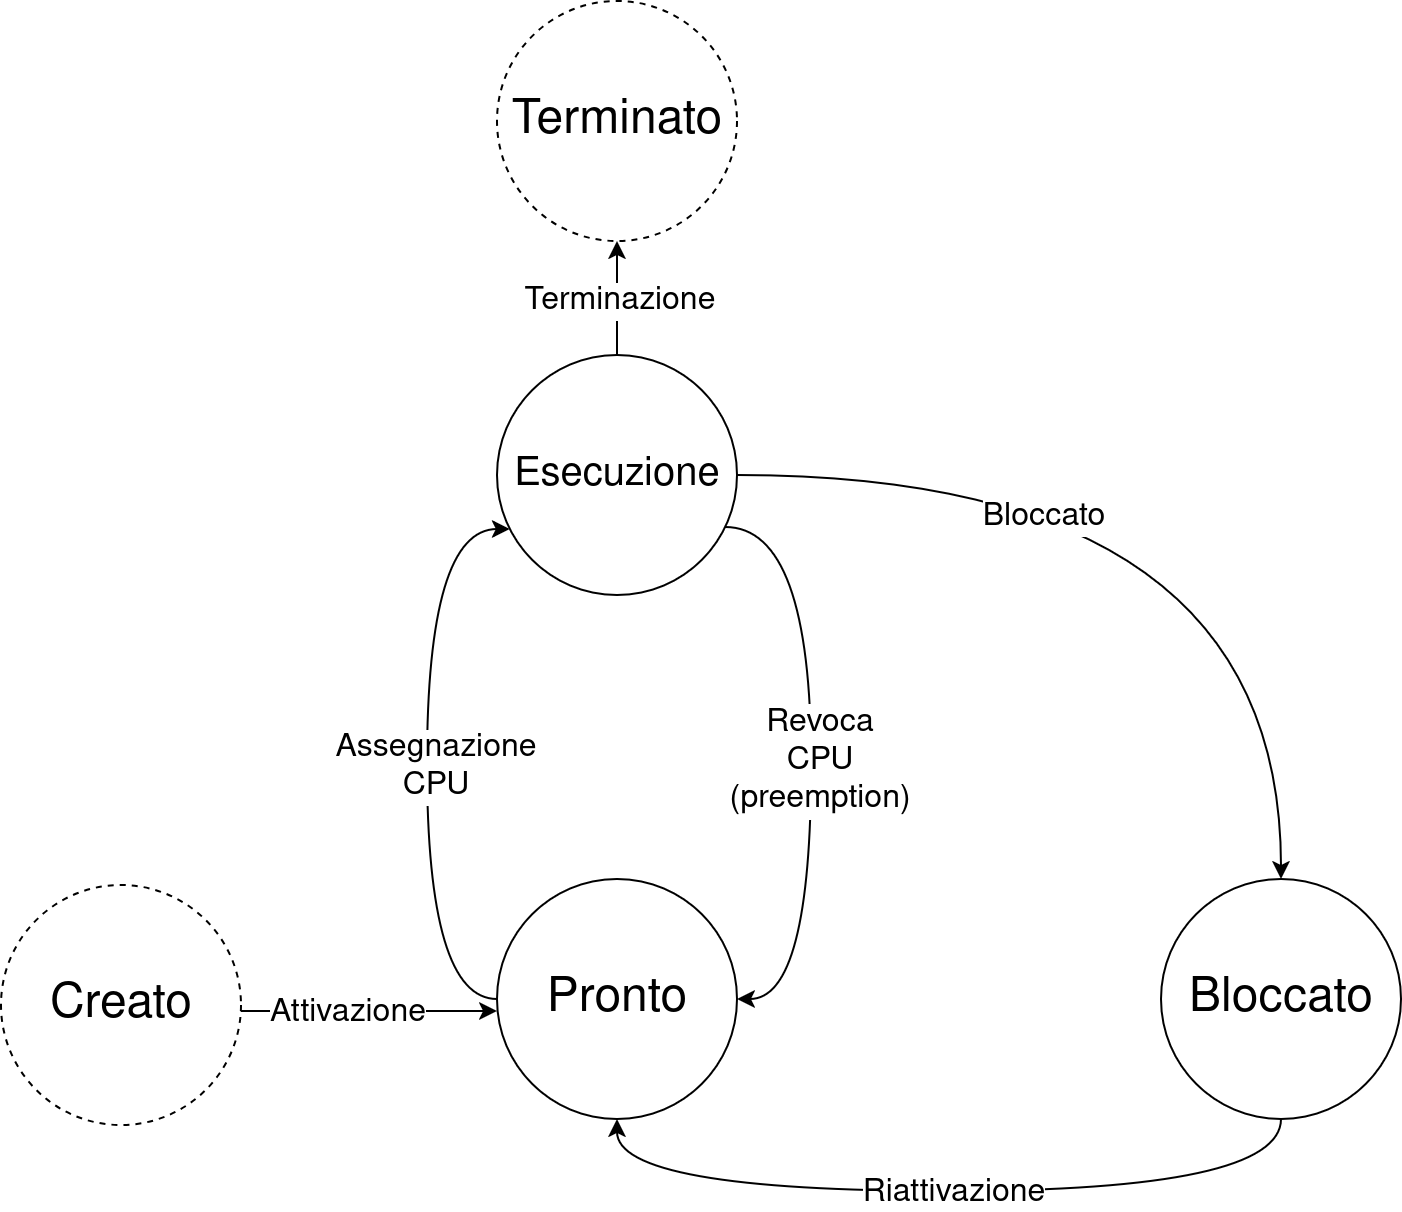
\includegraphics[scale=0.25]{../figures/thread_stati.png}
\end{center}

In Java le transizioni fra stati possono corrispondere a particolari chiamate di metodi da dentro l'oggetto thread.
In particolare:
\begin{itemize}
	\item \textit{Pronto}: il thread arriva qui quando si chiama il metodo \lstinline|start()|, e può tornarci alla fine del quanto di tempo assegnatogli, per \textit{preemption}, o per concessione volontaria (attraverso \lstinline|Thread.yield()|).

		Inoltre, torna qui se era bloccato e viene sbloccato (fine \lstinline|sleep()|, \lstinline|notify()|, blocchi su risorse rilasciati, ecc...);
	\item \textit{Bloccato}: un thread arriva qui quando effettua una sospensione volontaria (\lstinline|sleep()|, \lstinline|wait()|, blocchi \lstinline|synchronized|) o quando viene bloccato involontariamente su risorse (file, I/O, ecc...);
	\item \textit{Esecuzione}: questo è lo stato in cui il thread effettivamente esegue.
\end{itemize}

\subsubsection{Thread e S/O}
Il concetto di thread in Java è chiaramente parallelo a quello di thread nei S/O.

Vediamo una breve outline cronologica di questa relazione: 
\begin{itemize}
	\item 
Oggi la prassi è quella di associare ad ogni thread Java un thread di S/O, e lasciare che siano i meccanismi di gestione dei processi del S/O a gestire i thread Java in esecuzione;

\item
Storicamente, questo non è stato sempre il caso: le prime JVM erano infatti processi monolitici, con un unico flusso di esecuzione, che gestivano internamente tutti i diversi thread.
\end{itemize}

In ogni caso, le specifiche del linguaggio si dimostrano (volutamente) blande sull'argomento thread, in quanto la maggior parte delle problematiche associate alla gestione di questi è associata alla struttura specifica del S/O.

\subsubsection{Priorità thread}
Di un thread Java si può impostare la priorità (un numero da 1 a 10, via \lstinline|setPriority(int prio)|), e questa dovrebbe grossomodo corrispondere alla priorità del corrispondente thread S/O (grossomodo in quanto l'S/O potrebbe prevedere più di 10 livelli di priorità).

Per questo motivo, bisognerebbe usare la priorità dei thread Java solo come indicazione per il S/O e come ottimizzazione, e non fidarsi completamente di ottenere del comportamento sperabile. 

Il thread di default parte con priorità normale (il valore medio, cioè 5).
Quando si creano nuovi thread, questi ereditano la priorità del thread padre (quindi 5 dal thread di default).

La schedulazione dei thread Java è in genere di tipo \textit{fixed priority}. 

\subsubsection{Terminare e riattivare thread}
Quando un thread termina, non si può usare nuovamente \lstinline|start()| per rimetterlo in esecuzione, ma bisogna crearne una nuova istanza ed eseguire quella.

Se da un thread si vuole terminare l'esecuzione del solo thread, si può chiaramente ritornare da \lstinline|run()|. Se si vuole invece terminare l'esecuzione dell'intero programma, si può usare \lstinline|System.exit()|. 

\subsubsection{Metodo sleep}
Il metodo \lstinline|sleep(long t)| permette di sospendere il thread per il numero di millisecondi specificato in \lstinline|t|.

Il metodo può lanciare l'eccezione \textit{InterruptedException}, e questo accade quando il thread viene interrotto.
Per questo bisogna definire un blocco \lstinline|catch| che catturi tale eccezione e fornisca un qualche tipo di handler:
\begin{lstlisting}[language=java, style=codestyle]	
void run() {
	while(true) {
		System.out.println("Tick");
		try {
			Thread.sleep(1000);
		} catch(InterruptedException e) {
			System.err.println("Il thread e' stato svegliato. " + e.getMessage());
		}
	}
}
\end{lstlisting}

\subsection{Corse critiche}
Un problema in cui si può incorrere quando si sfruttano i thread è quello delle \textbf{corse critiche}.

Quando più thread interagiscono con lo stesso oggetto, infatti, potrebbero lasciarlo in stati inconsistenti a causa di scritture contemporanee che si cancellano fra di loro.
In altre parole, le operazioni su campi di oggetti in Java non sono (di default) \textit{atomiche}, e i metodi che le implementano possono essere deschedulati (per preemption) quando l'oggetto su cui stanno lavorando è ancora in stato inconsistente.

\subsubsection{Monitor, metodi \lstinline|synchronized|}
In Java questo problema viene risolto sfruttando il modello dei \textbf{monitor}.
Secondo questo modello, ad ogni oggetto è associato un \textbf{lock}, che può essere \textit{aperto} o \textit{chiuso}.

Per agire su un oggetto, un thread deve acquisire un lock.
Quando avrà finito la sua operazione, potrà rilasciare tale lock.

Dal punto di vista sintattico, questo si implementa usando il modificatore (applicabile ai metodi) \lstinline|synchronized|.
Quando un thread esegue un metodo \lstinline|synchronized| e agisce su un'oggetto $x$, quello che accade è:
\begin{itemize}
	\item Acquisisce il lock di $x$;
	\item Esegue il corpo del metodo ;
	\item Rilascia il lock di $x$.
\end{itemize}

Tutti i metodi dichiarati come \lstinline|synchronized| condividono per ciascun oggetto un lock (il lock predefinito).
I metodi non \lstinline|synchronized| possono invece bypassare il meccanismo dei lock, anche quando un metodo che invece è \lstinline|synchronized| ha il lock sull'oggetto cercato.

Per questo è importante dichiarare come \lstinline|synchronized| tutti i metodi che rischiano di portare oggetti in stati inconsistenti.
Di contro, è abbastanza naturale definire metodi che non richiedono di rispettare i lock (metodi non bloccanti, di lettura, ecc...). 

Abbiamo quindi che i metodi \lstinline|synchronied| \textit{cercano} di ottenere i lock sugli oggetti che modificano.
I lock si acquisiscono per conto del thread corrente: se quel thread è già in possesso del lock cercato, non si blocca e va direttamente all'esecuzione del metodo.

Nel caso di metodi \lstinline|synchronized| il lock viene rilasciato:
\begin{itemize}
	\item Al normale termine del esecuzione del metodo;
	\item In caso di situazioni particolari come le eccezioni.
\end{itemize}

\subsubsection{Blocchi \lstinline|synchronized|}
La parola chiave \lstinline|synchronized| può essere usata anche per definire \textit{blocchi} di codice, e non solo metodi.
In questo caso tali blocchi si comportano esattamente come i metodi che abbiamo descritto finora.

I blocchi sincronizzati accettano un argomento, che è quello su cui vogliamo bloccare.
Nel caso di metodi sincronizzati, l'oggetto è implicitamente la classe del metodo:
\begin{lstlisting}[language=java, style=codestyle]	
class A {
	void synchronized foo() {
		// sincronizza su A
	}

	void bar() {
		synchronized(this) {
			// come sopra ma inutilmente esplicito
		}
	}
}
\end{lstlisting}
Coi blocchi sincronizzati si possono però avere altri oggetti su cui sincronizzare. Il loro uso è quindi necessario quando:
\begin{itemize}
	\item Non tutto il codice di un metodo deve essere eseguito in mutua esclusione (sincronizzato). Questo è particolarmente utile aumentare il grado di parallelismo dei thread: se si sincronizza solo quando gli oggetti effettivamente ci servono, si lascia tempo agli altri thread per lavorare sullo stesso oggetto; 
	\item Si vuole sincronizzare su oggetti diversi da quello implicito. Ad esempio, si potrebbe voler dire:
\begin{lstlisting}[language=java, style=codestyle]	
void metodo(Parametro p) {
	synchronized(p) {
		// qui abbiamo il lock su p
	}
}
\end{lstlisting}

In questo caso l'oggetto di cui si prende il lock non è più la classe corrente, ma l'oggetto di tipo \textit{Parametro} che passiamo nell'argomento $p$.

Questo può essere utile quando si usano oggetti che non prevedono la sincronizzazione di default: in questo modo imponiamo \textit{noi} che le operazioni che svolgiamo vengano sincronizzate; 

	\item Si vuole sincronizzare su un array. Questo in quanto le array non possono essere soggetto di lock impliciti (non sono classi che definiscono metodi).
		La sintassi è in questo caso analoga all'esempio precedente.
\end{itemize}

Più lock su più oggetti possono essere ottenuti innestando blocchi \lstinline|synchronized|.

\subsubsection{Lock statici}
Quando il modificatore \lstinline|synchronized| viene usato su metodi statici il lock implicito non è sull'\textit{istanza} di classe, ma sull'intera classe. In questo modo si possono definire metodi che esegono in maniera mutualmente esclusiva sull'intero oggetto classe.

\subsection{Deadlock}
Nel caso due thread debbano ottenere un lock appartenente all'altro per portare avanti la loro operazione, e non siano ancora in condizioni di rilasciare il loro lock, si incorre in una situazione detta \textbf{deadlock}.

Un risultato teorico è che \textit{se si prendono i lock sempre nello stesso ordine}, i deadlock non possono verificarsi. Questo chiaramente non è sempre facile dal punto di vista implementativo.

\subsection{Sincronizazzione}
Veniamo a come eseguire operazioni in thread solo nella condizione che un altro thread abbia eseguito la sua operazione.
Questo è un problema di \textit{sincronizzazione} o in particolare di \textbf{comunicazione} fra thread.

Facciamo attenzione al fatto che la parola chiave \lstinline|synchronized| è fuorviante: in verità questa risolve un problema di \textit{interferenza}, o più propriamente di \textbf{mutua esclusione} dell'accesso a determinate risorse.

Il problema che vogliamo invece risolvere adesso è di \textit{sincronizzazione} temporale nell'esecuzione di operazioni in stretto ordine cronologico.

In Java questo problema viene risolto sfruttando metodi definiti direttamente sulla classe \textit{Object}:
\begin{itemize}
	\item \lstinline|notify()|: permette di \textit{notificare}, appunto, un oggetto nel \textit{wait-set} dell'oggetto che lo chiama (più dettagli in seguito);
	\item \lstinline|notifyAll()|: come sopra, ma notifica tutti gli oggetti nel \textit{wait-set}; 
	\item \lstinline|wait()|: permette di sospendere l'esecuzione di un thread fino al verificarsi di una determinata condizione (notificata da qualcun'altro). Questo è un metodo che non restituisce nulla ma può lanciare la \textit{InterruptedException}.
		Quando si chiama \lstinline|wait()| i lock dell'oggetto vengono rilasciati e acquisiti automaticamente al rientro in esecuzione.

		Ad ogni oggetto è associato un \textit{wait-set}. Quando si chiama wait su un oggetto il thread viene sospeso e inserito nel \textit{wait-set} di quell'oggetto.
		Quando il \textit{wait-set} riceve una notifica con \lstinline|notify()|, uno degli oggetti in attesa viene risvegliato e messo in coda pronti.
		Se invece la notifica è con \lstinline|notifyAll()|, vengono risvegliati tutti.
\end{itemize}

\end{document}
